\section{Experimental results}


\subsection{Space-Only modulation}

\begin{frame}{Space-Only modulation}

    \begin{columns}[c, onlytextwidth]

        \begin{column}{0.55\textwidth}

            In the case of space-only modulation, piezoelectric patches can be either in the short-circuit (ON) or open-circuit (OFF) state.
            Three different configurations of the ST cell are considered:

            \begin{itemize}
                \item \textit{OFF-OFF-OFF}
                \item \textit{ON-ON-ON}
                \item \textit{ON-OFF-OFF}
            \end{itemize}

        \end{column}

        \begin{column}{0.45\textwidth}

            \begin{figure}[H]
                \centering
                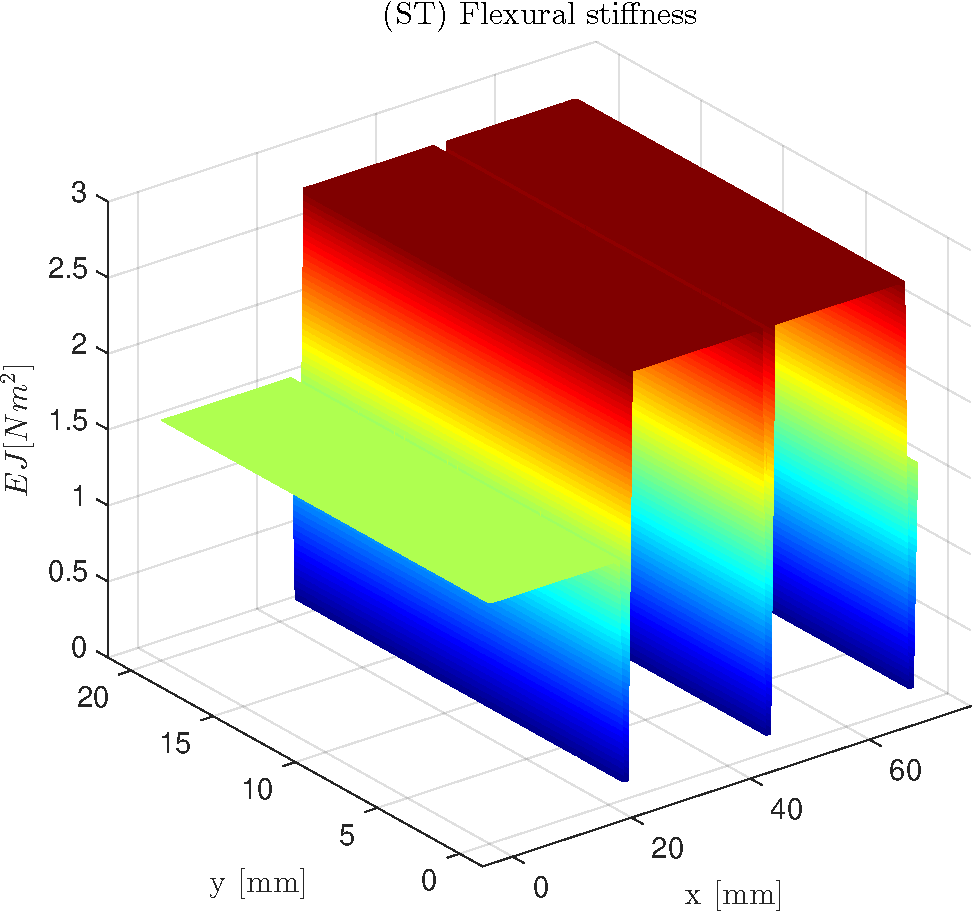
\includegraphics[width=0.9\textwidth]{img/MATLAB/ST_cell_ON-OFF-OFF.pdf}
                \caption{ST cell in the case \textit{ON-OFF-OFF}.}
            \end{figure}

        \end{column}

    \end{columns}

    \vspace{9pt}

    Numerical simulations performed using TMM\footnotemark[1] and PWEM\footnotemark[2] are compared against experimental data.
    \texttt{Comsol Multiphysics} is also adopted as a valid reference.

    \footnotetext[1]{Transfer Matrix Method}
    \footnotetext[2]{Plane Wave Expansion Method}

\end{frame}



\begin{frame}{Case \textit{OFF-OFF-OFF}}

    The first band-gap is observed at $f_{BG}^{OFF-OFF-OFF} = [3.8, 7.5] kHz$.

    \begin{figure}[H]
        \centering
        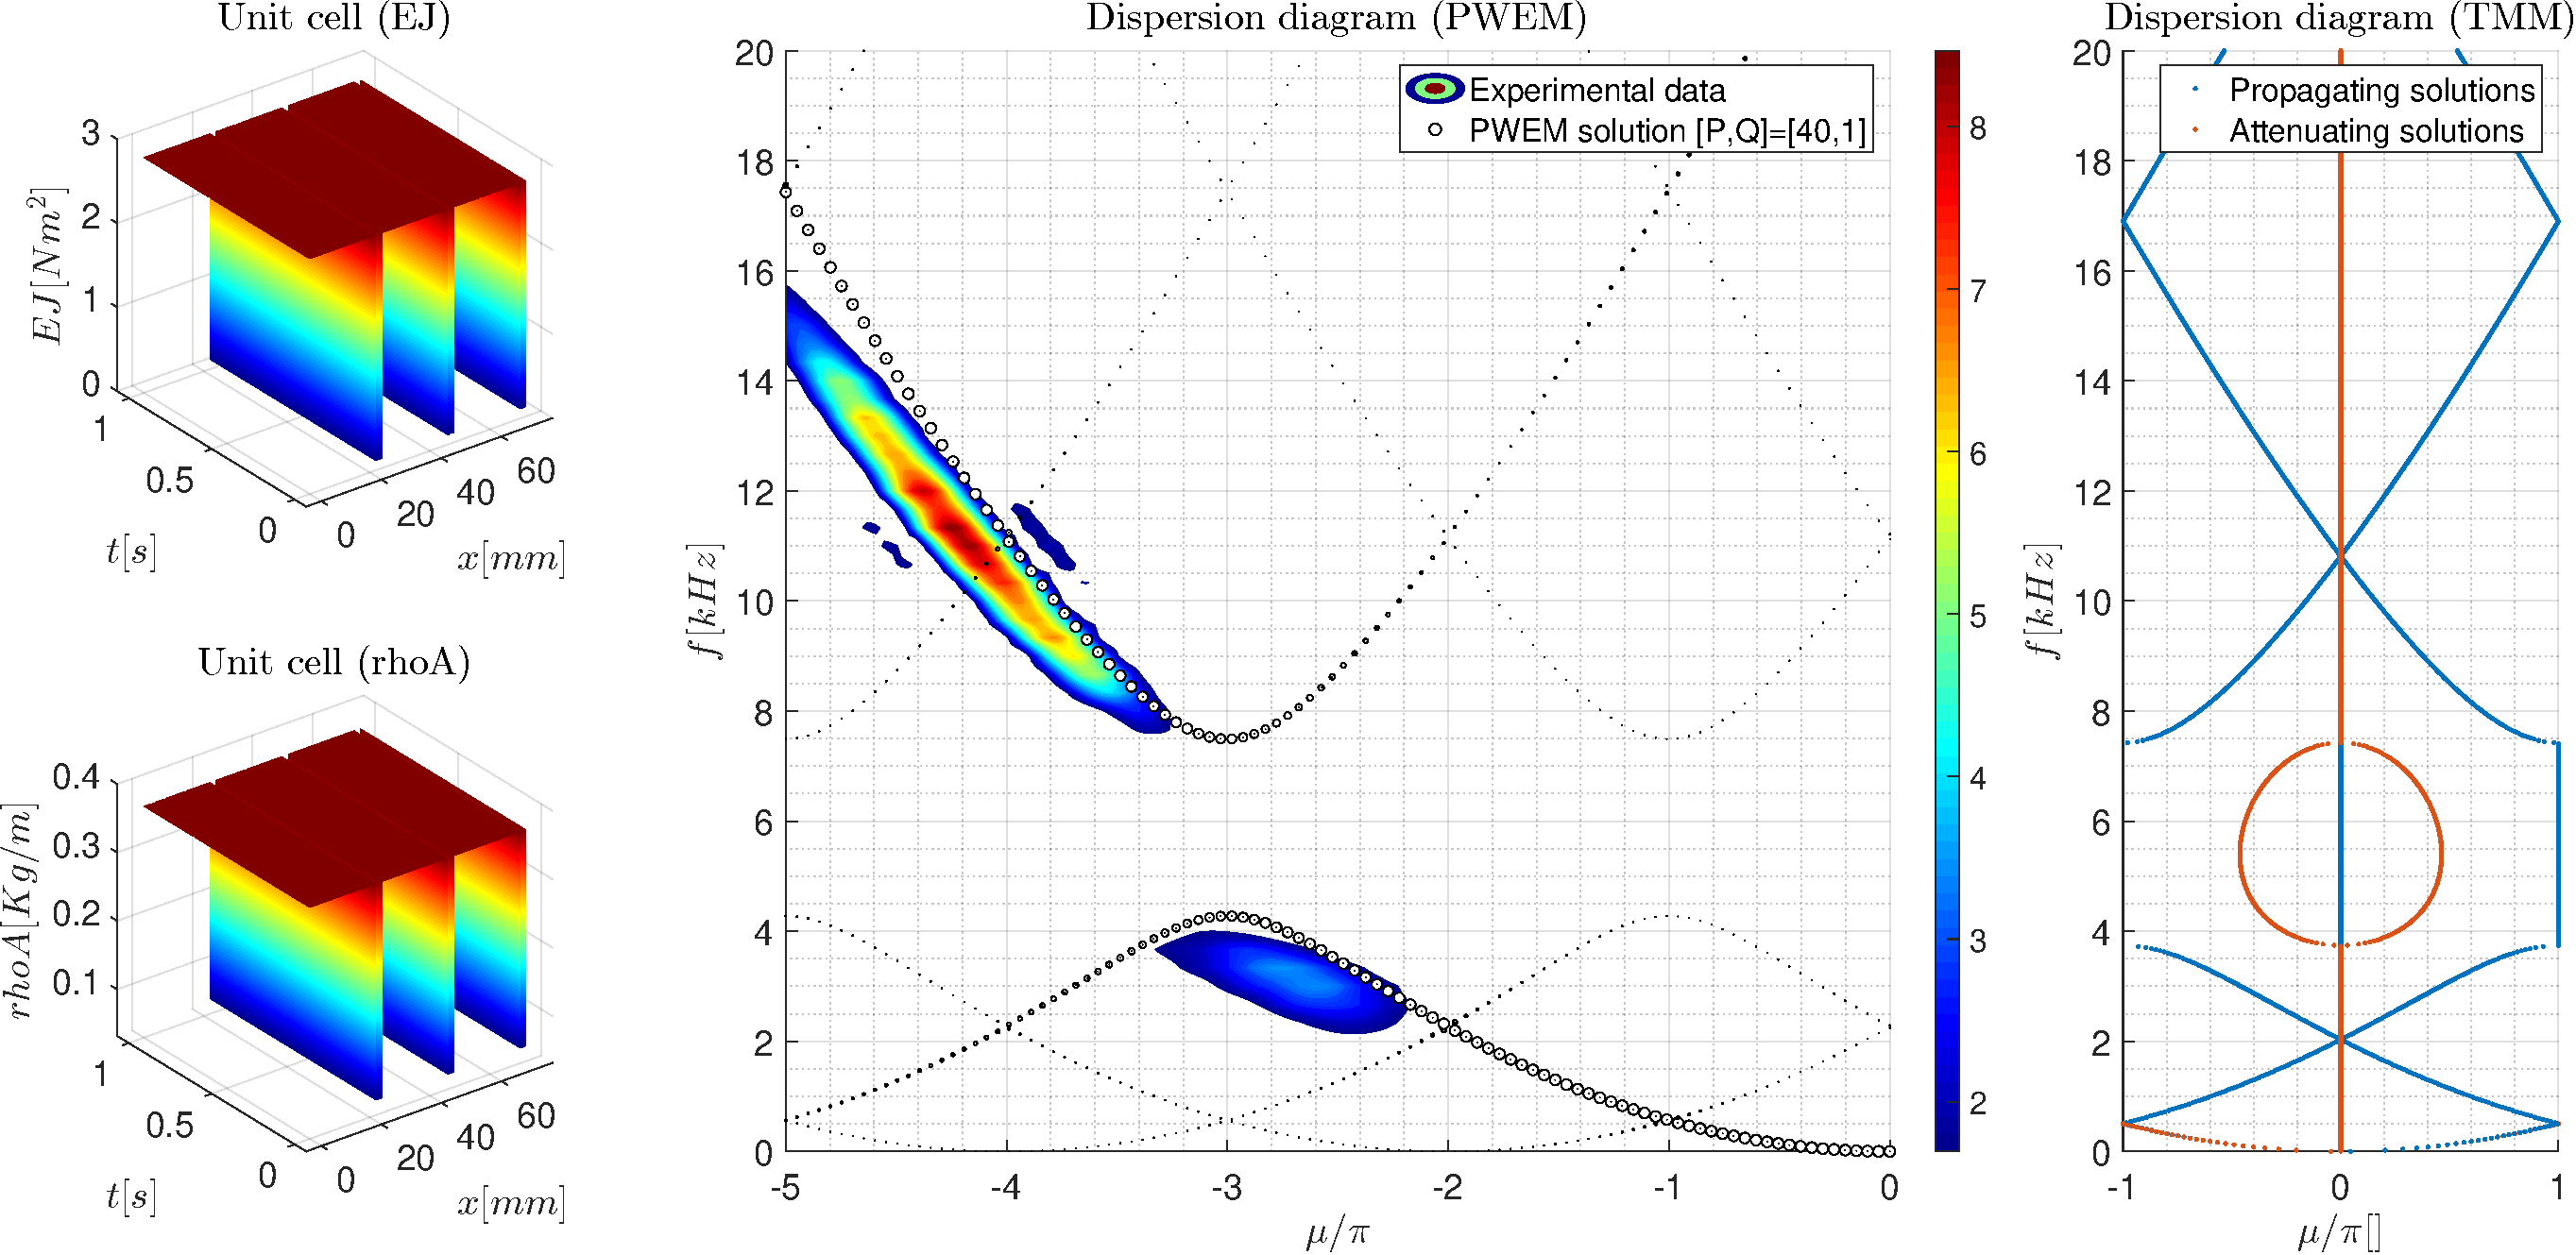
\includegraphics[width=\textwidth]{./img/MATLAB/PWEM_TMM_EXP OFF-OFF-OFF @0kHz.pdf}
        \caption{Dispersion diagram for the OFF-OFF-OFF configuration.}
    \end{figure}

\end{frame}



\begin{frame}{Case \textit{ON-ON-ON}}

    Short-circuiting all the piezoelectric patches results in a decrease of the structural stiffness and a shift of the band-gap towards lower frequencies ($f_{BG}^{ON-ON-ON} = [3.4, 5.6] kHz$).

    \begin{figure}[H]
        \centering
        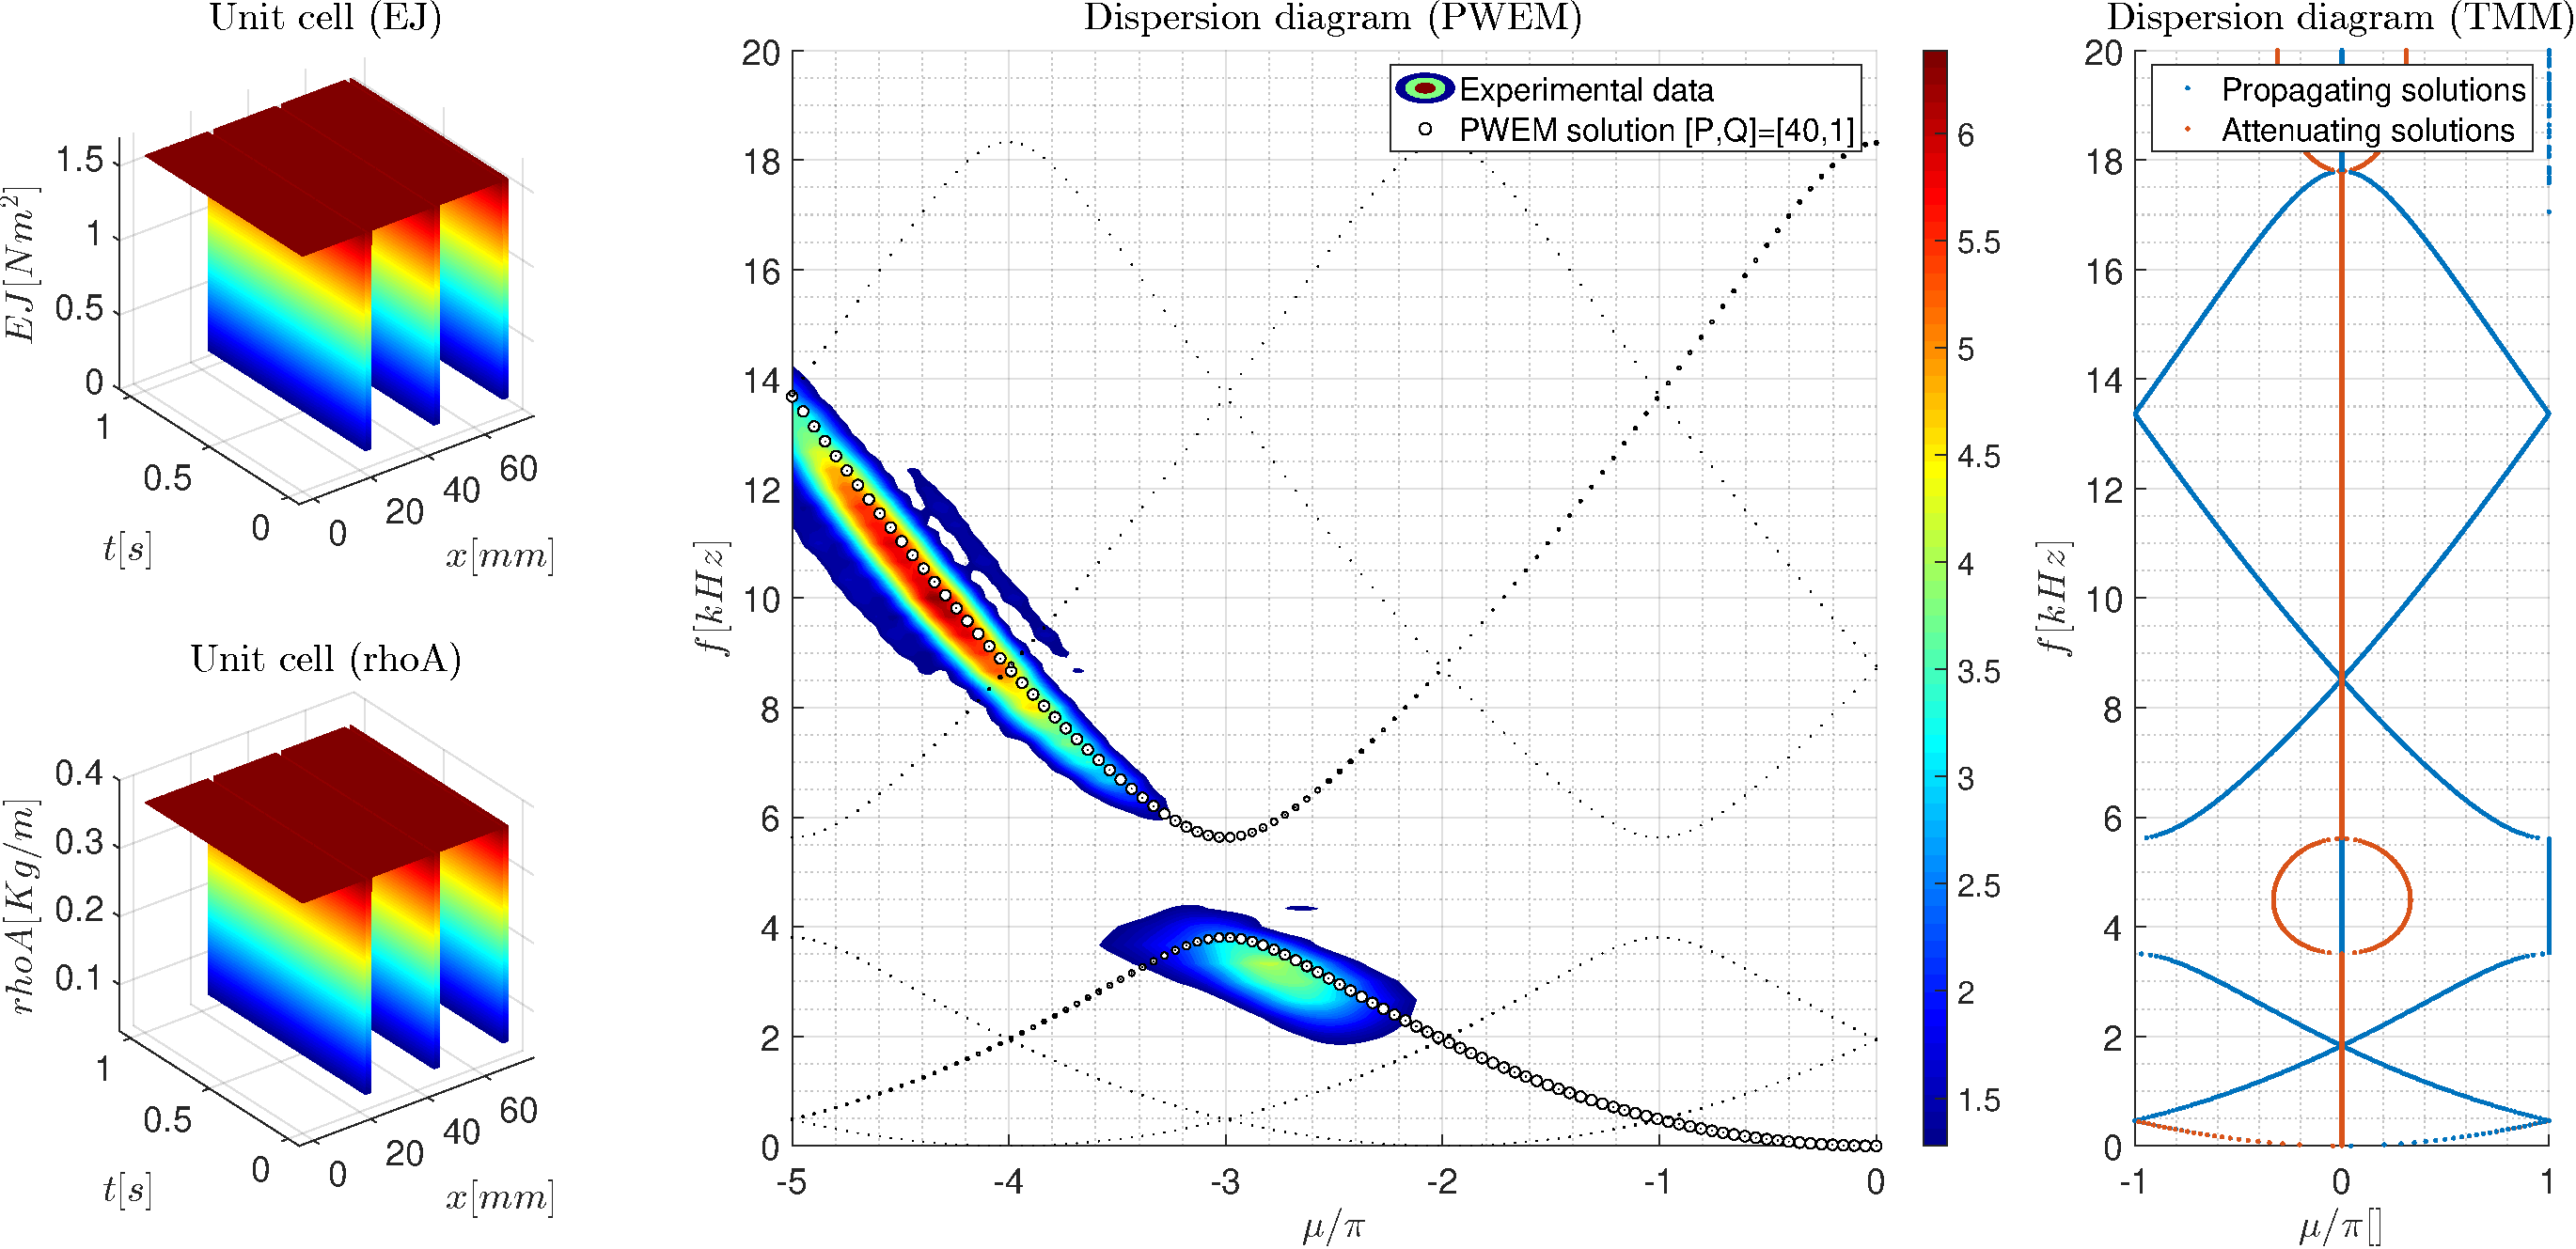
\includegraphics[width=\textwidth]{./img/MATLAB/PWEM_TMM_EXP ON-ON-ON @0kHz.pdf}
        \caption{Dispersion diagram for the ON-ON-ON configuration.}
    \end{figure}

\end{frame}



\begin{frame}{Case \textit{ON-OFF-OFF}}

    The introduction of additional sources of dispersion in the system results in a higher number of band-gaps visible in the same frequency range.

    \begin{figure}[H]
        \centering
        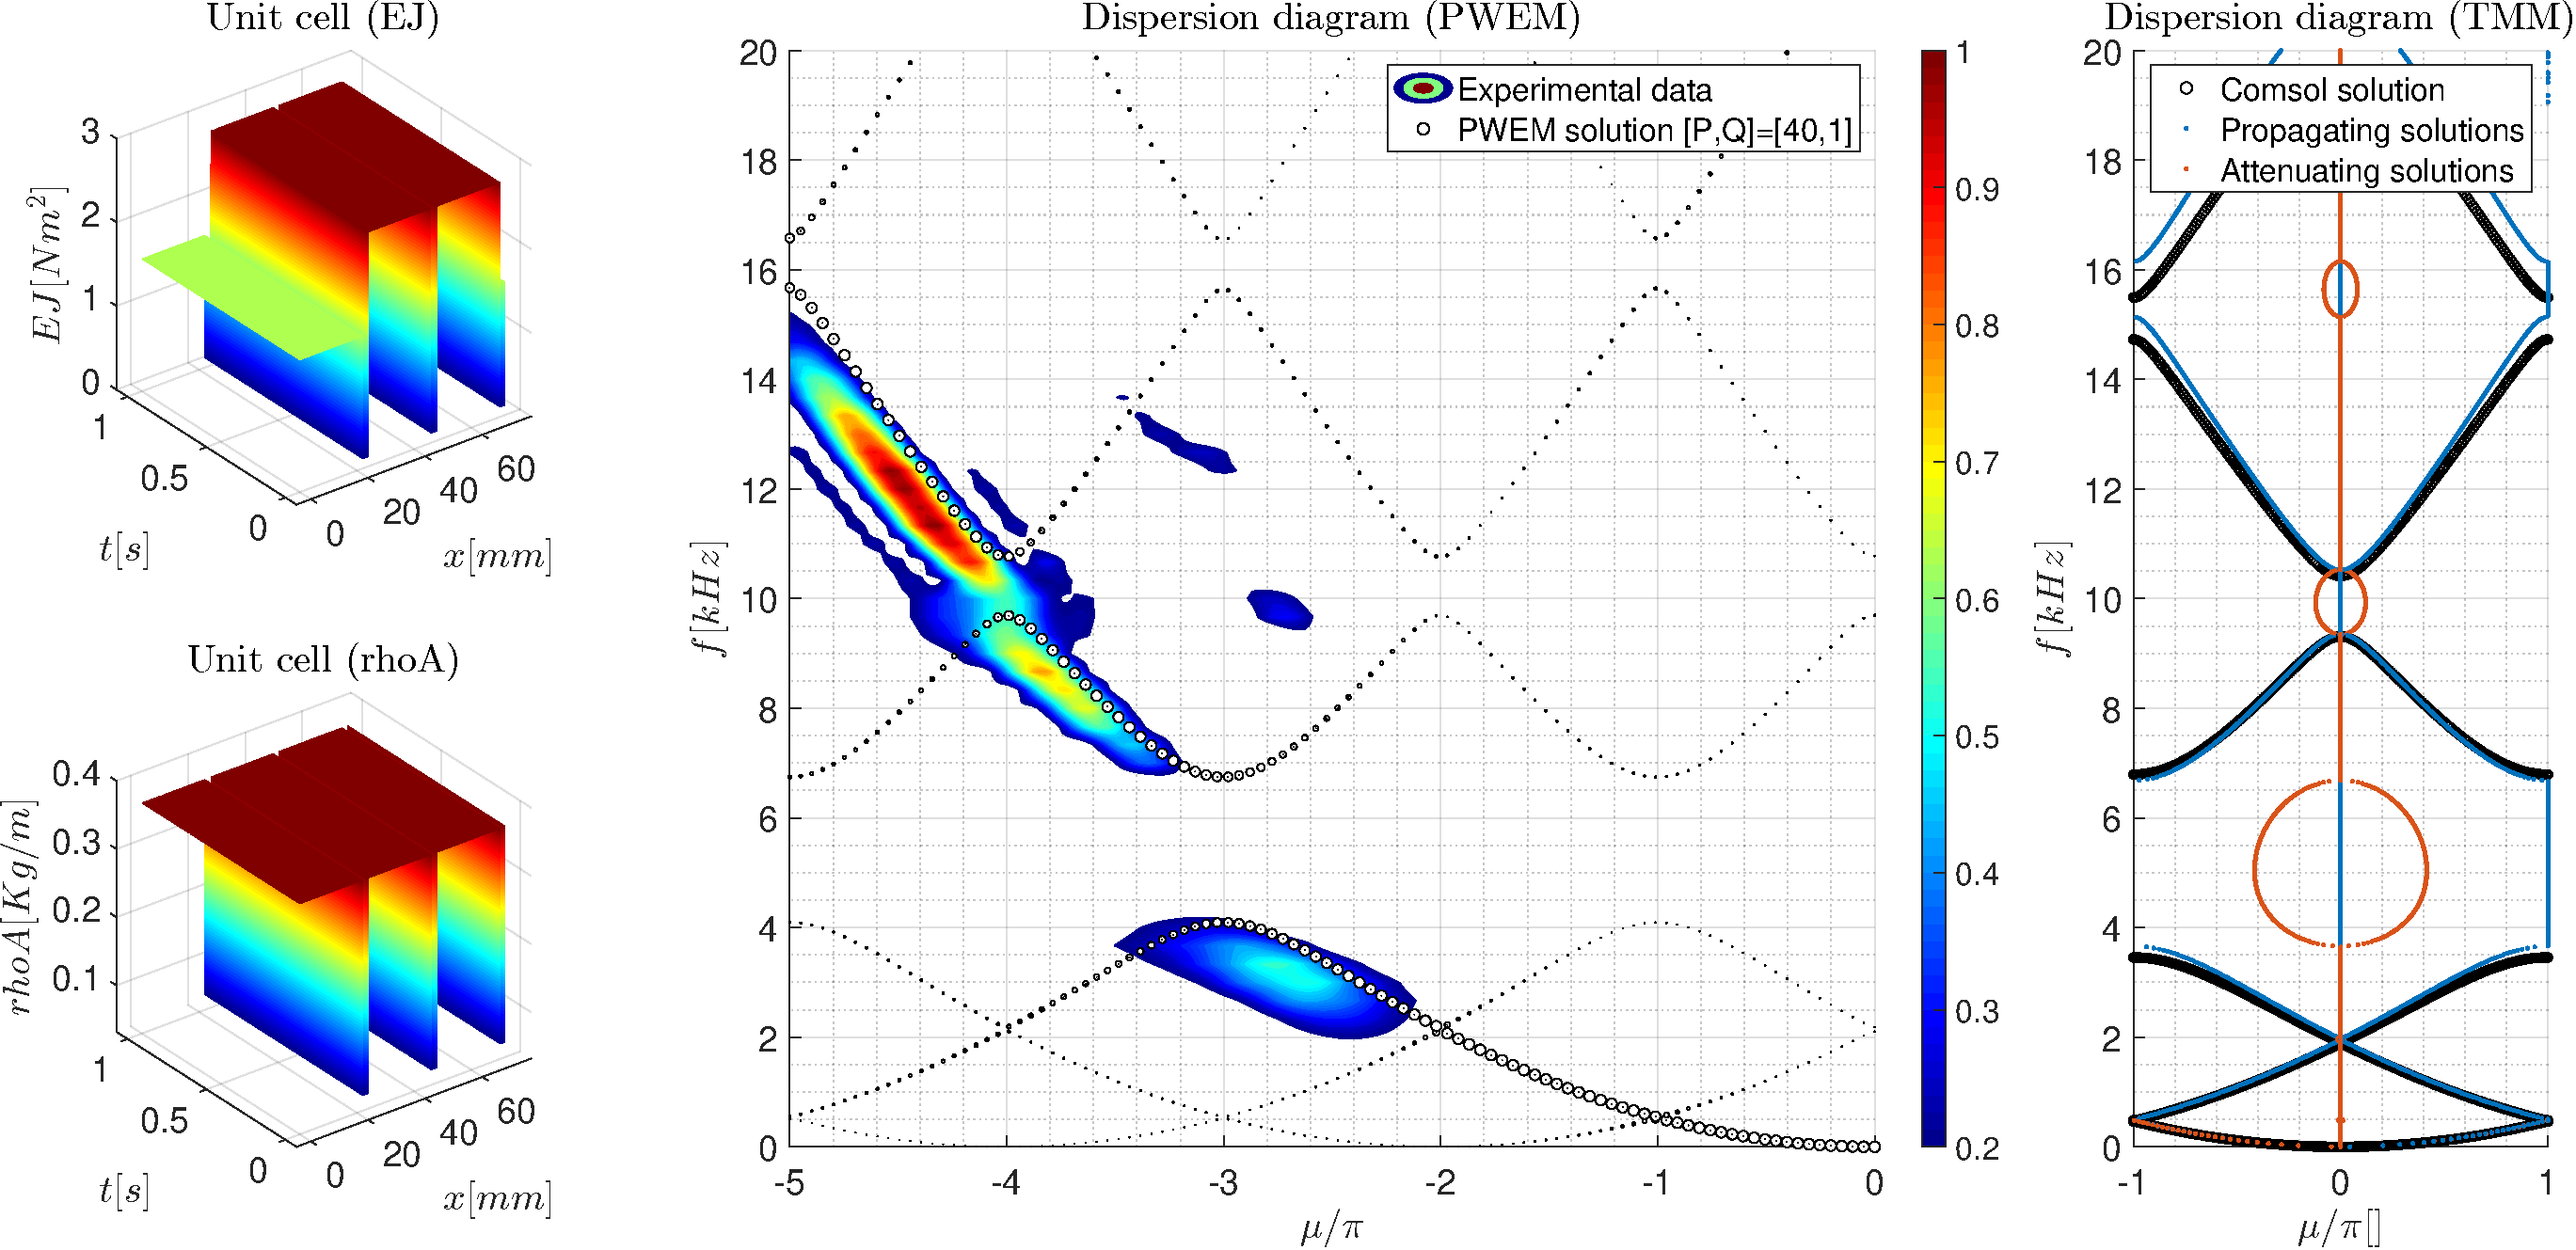
\includegraphics[width=\textwidth]{./img/MATLAB/PWEM_TMM_EXP ON-OFF-OFF @0kHz.pdf}
        \caption{Dispersion diagram for the ON-OFF-OFF configuration.}
    \end{figure}

\end{frame}



\subsection{Space-Time modulation}

\begin{frame}{Space-Time modulation}

    \begin{columns}[c, onlytextwidth]

        \begin{column}{0.55\textwidth}

            For the case of space-time modulations, piezoelectric patches are driven by equal (but phase-shifted) signals.
            Three different pairs of shunt modulation frequencies ($\pm f_m$) are considered.

            \vspace{9pt}

            PWEM numerical simulations are compared against experimental data.

        \end{column}

        \begin{column}{0.45\textwidth}

            \begin{figure}[H]
                \centering
                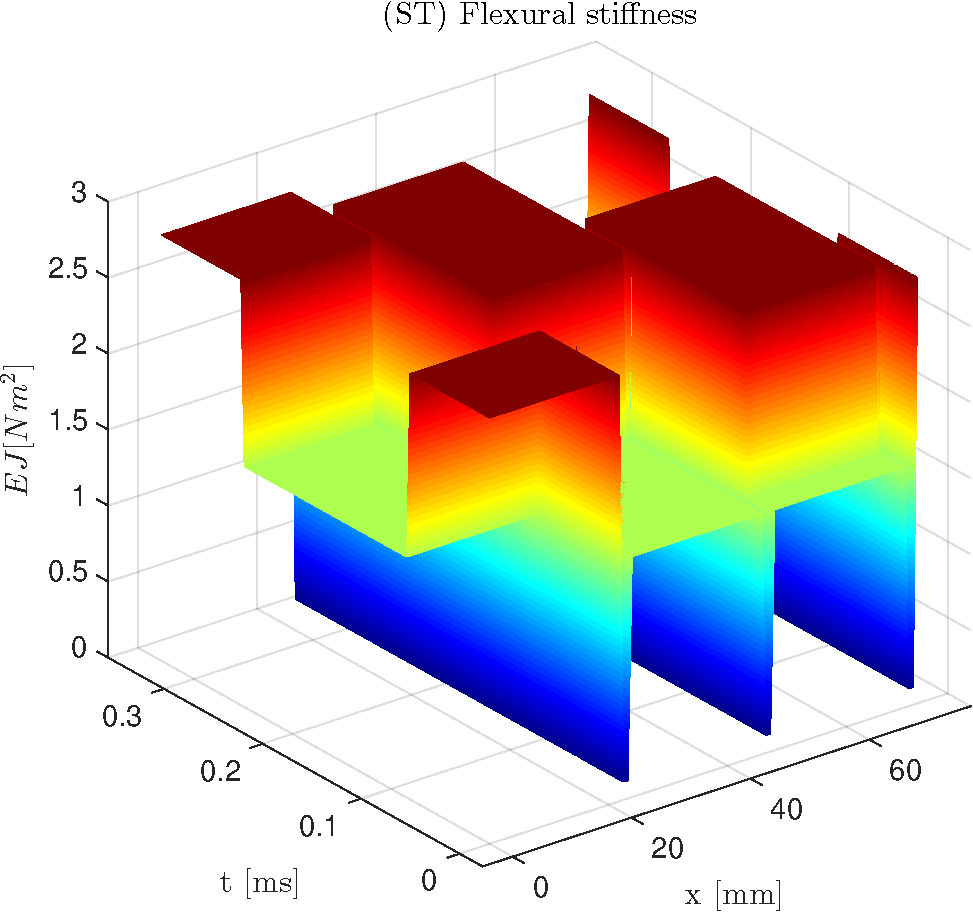
\includegraphics[width=0.9\textwidth]{img/MATLAB/ST_cell_Sinusoidal (discrete) @3kHz.pdf}
                \caption{ST cell in the case $f_m = 3 [Khz]$.}
            \end{figure}

        \end{column}

    \end{columns}

    The mechanical admittance of the $k$-th piezoelectric patch in the ST cell is given by:

    \begin{equation}
        Y_k^{SU} = \frac{(Y^{OFF} + Y^{ON})}{2} + \frac{(Y^{OFF} - Y^{ON})}{2} sign \left[ \cos \left( 2 \pi f_m t + (k-1) \frac{2\pi}{3} \right) \right]
    \end{equation}

\end{frame}



\begin{frame}{Modulation $f_m = \pm 1kHz$}


    Time modulation causes anti-symmetric dispersion diagrams and directional band-gaps to appear.
    This is a clear indication of the nonreciprocal behavior of the structure.

    A low frequency global band-gap is still present, associated with spatial modulation.

    \begin{figure}[H]
        \centering
        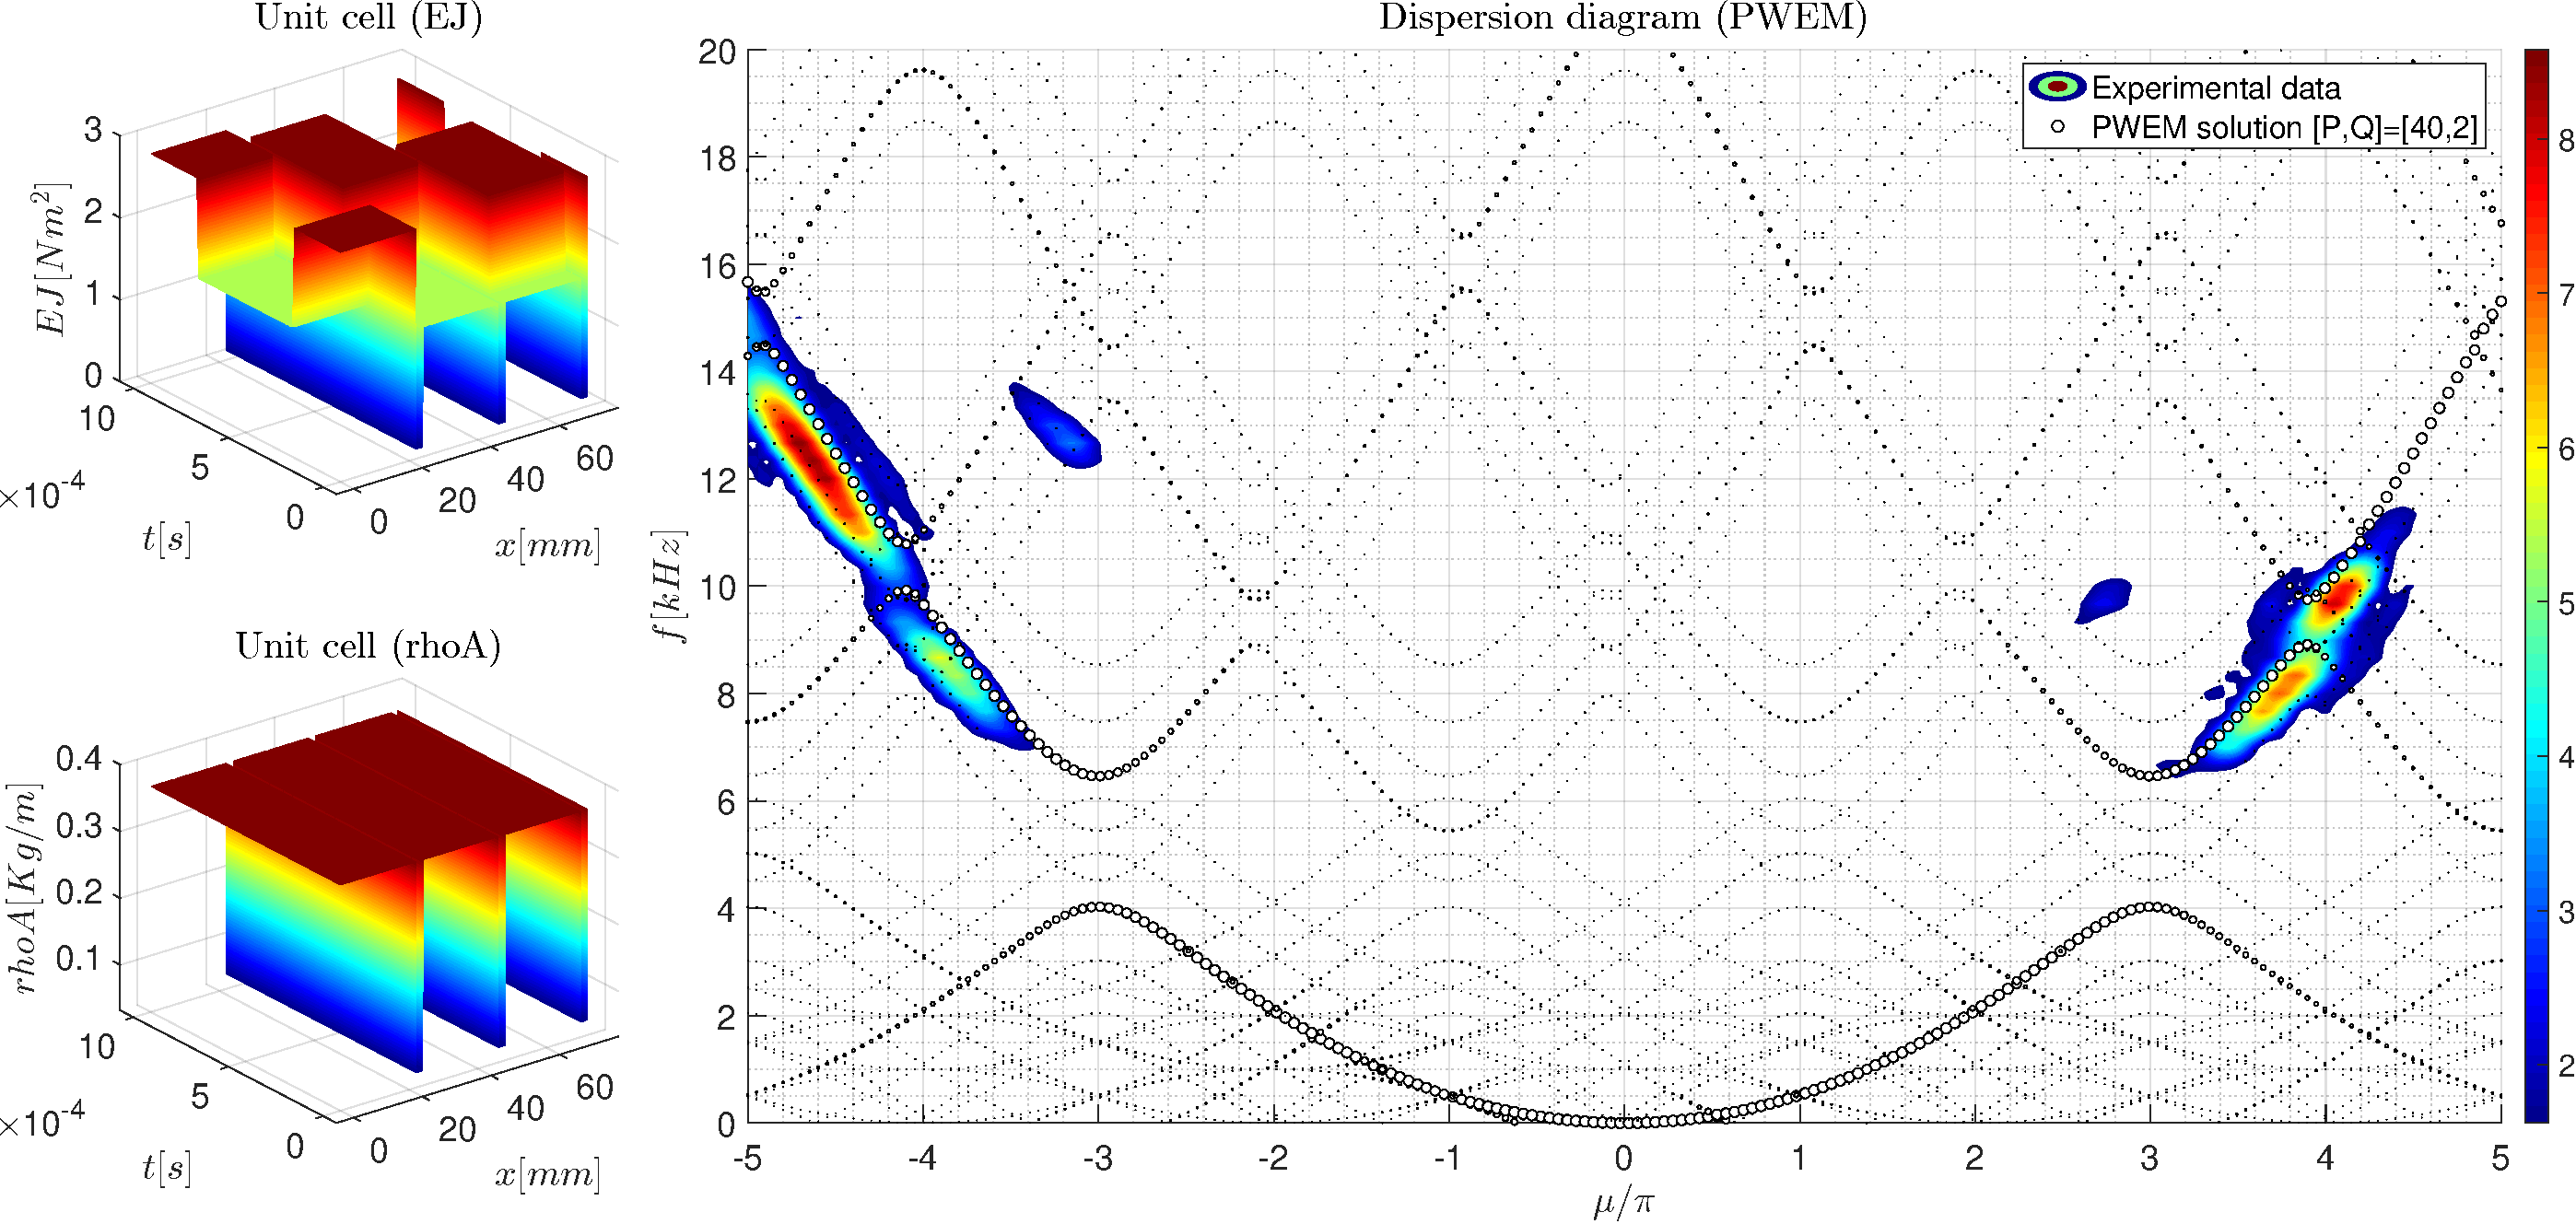
\includegraphics[width=\textwidth]{img/MATLAB/PWEM_EXP Sinusoidal (discrete) @1kHz.pdf}
        \caption{Dispersion diagram for the case of modulation frequency $f_m = \pm 1 kHz$.}
    \end{figure}

\end{frame}



\begin{frame}{Modulation $f_m = \pm 2kHz$}

    Intuitively, the phenomenon associated with the nonreciprocal behavior is now more pronounced, as the modulation frequency is doubled.
    Band-gap associated with space modulation seems to remain unchanged.

    \begin{figure}[H]
        \centering
        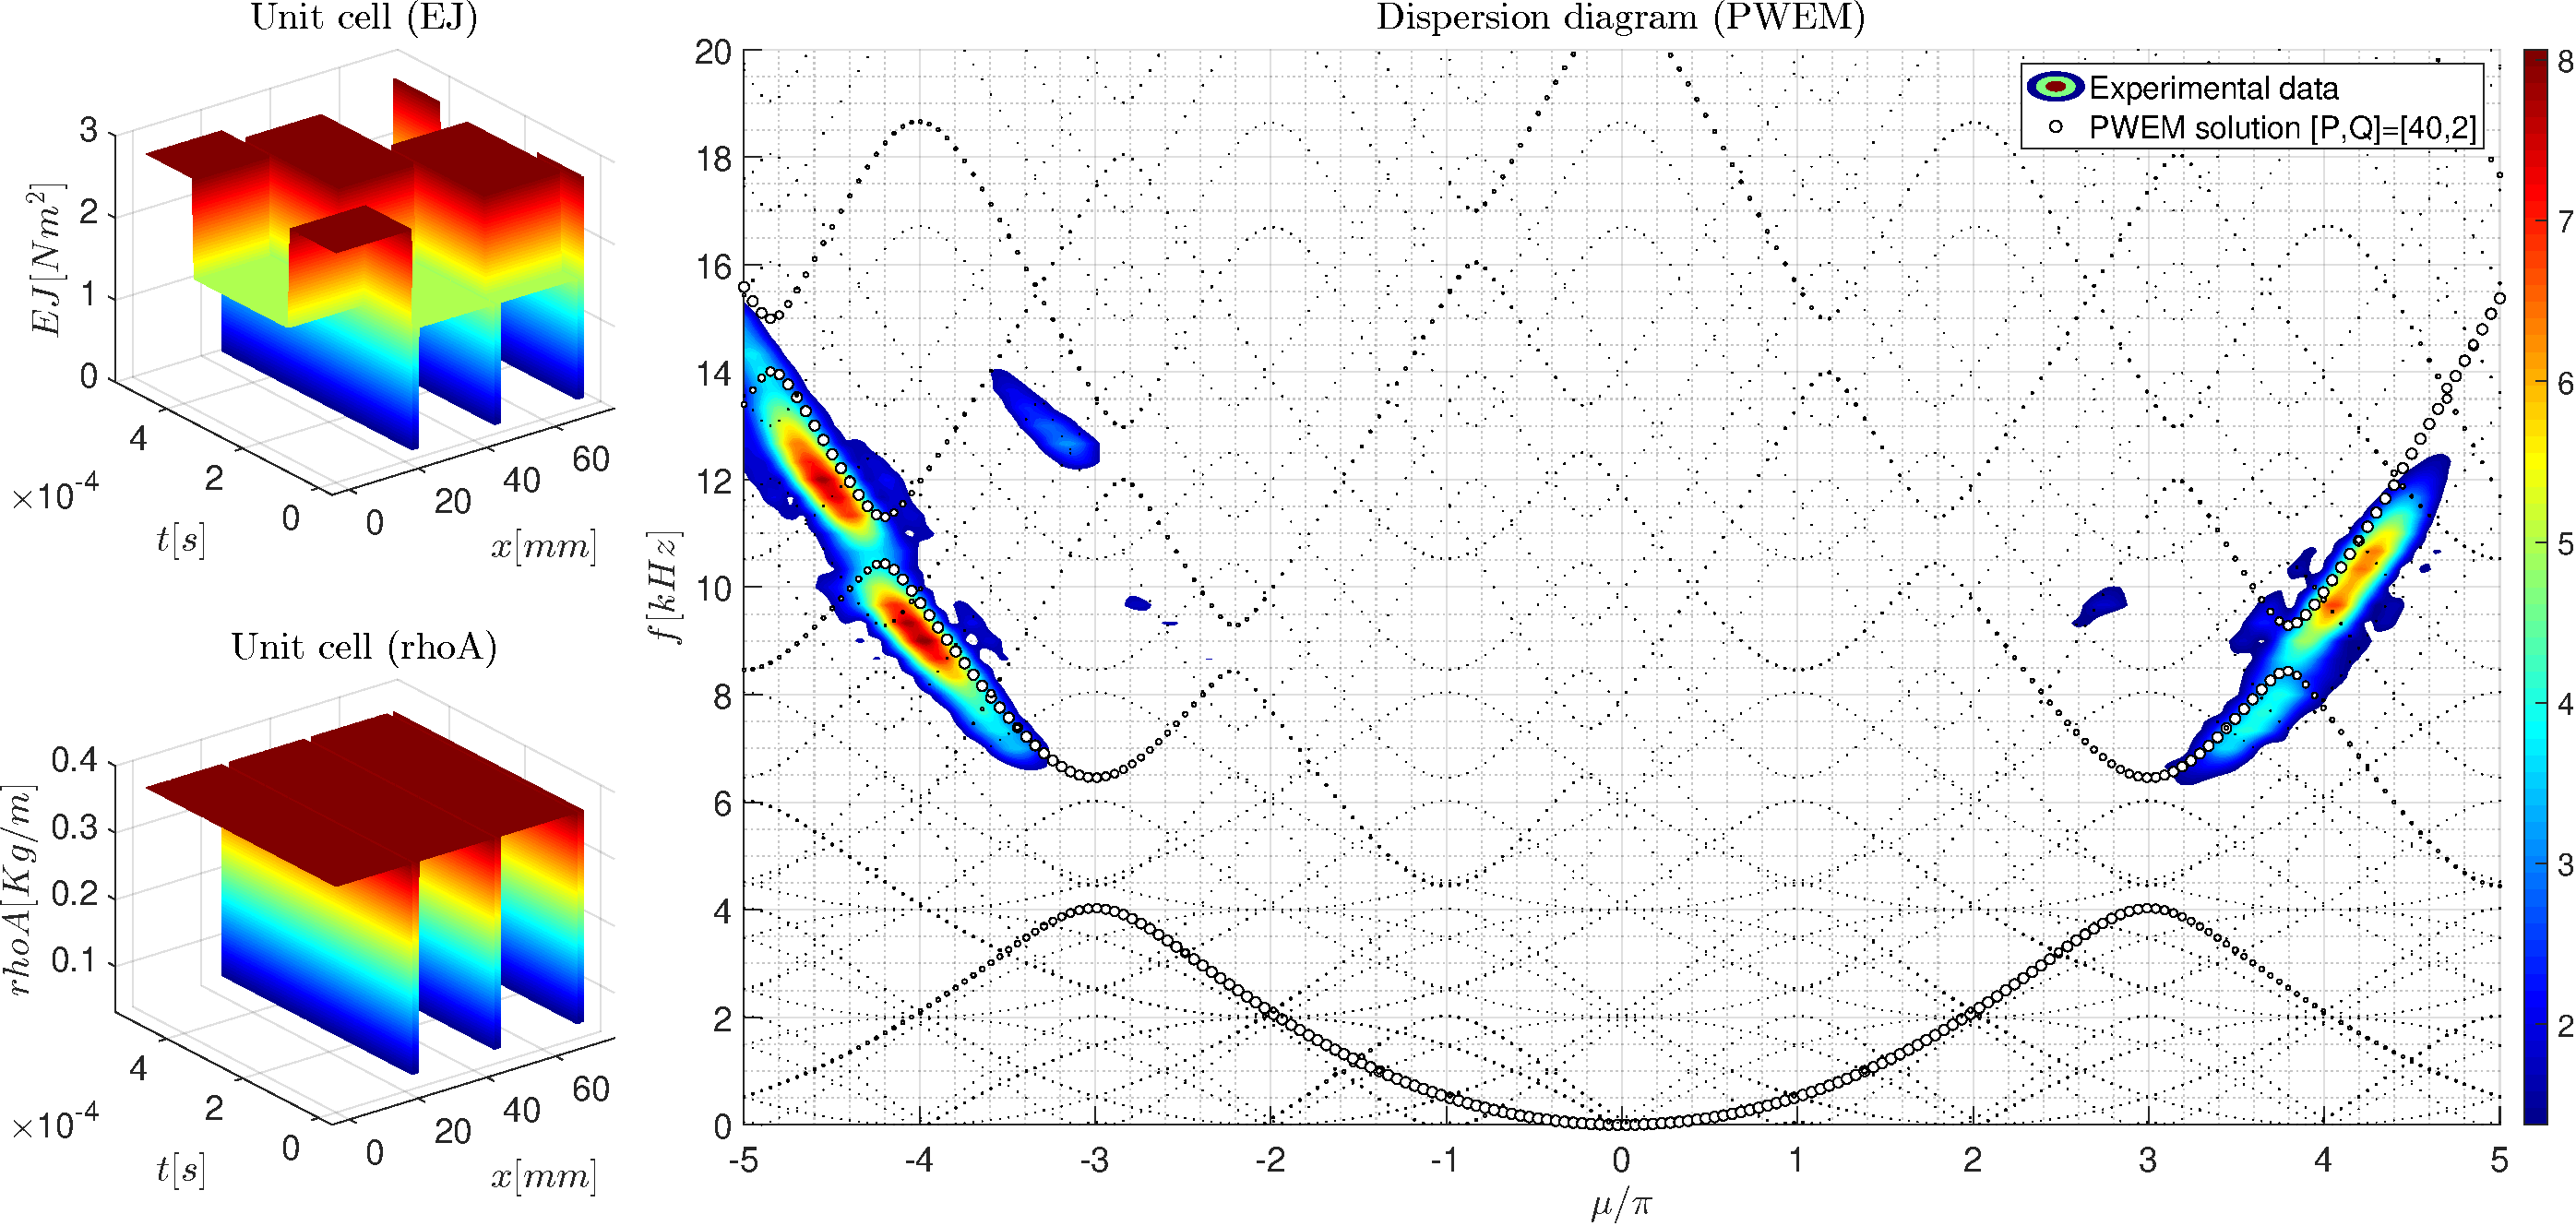
\includegraphics[width=\textwidth]{img/MATLAB/PWEM_EXP Sinusoidal (discrete) @2kHz.pdf}
        \caption{Dispersion diagram for the case of modulation frequency $f_m = \pm 2 kHz$.}
    \end{figure}


\end{frame}



\begin{frame}{Modulation $f_m = \pm 3kHz$}

    The asymmetrical shift of the already previously analyzed directional band-gaps is even more evident.
    With respect to the case $f_m = 0 kHz$ (\textit{ON-OFF-OFF}), a total shift of around $\pm1.5 kHz$ has been observed in the directional band-gaps positions.

    \begin{figure}[H]
        \centering
        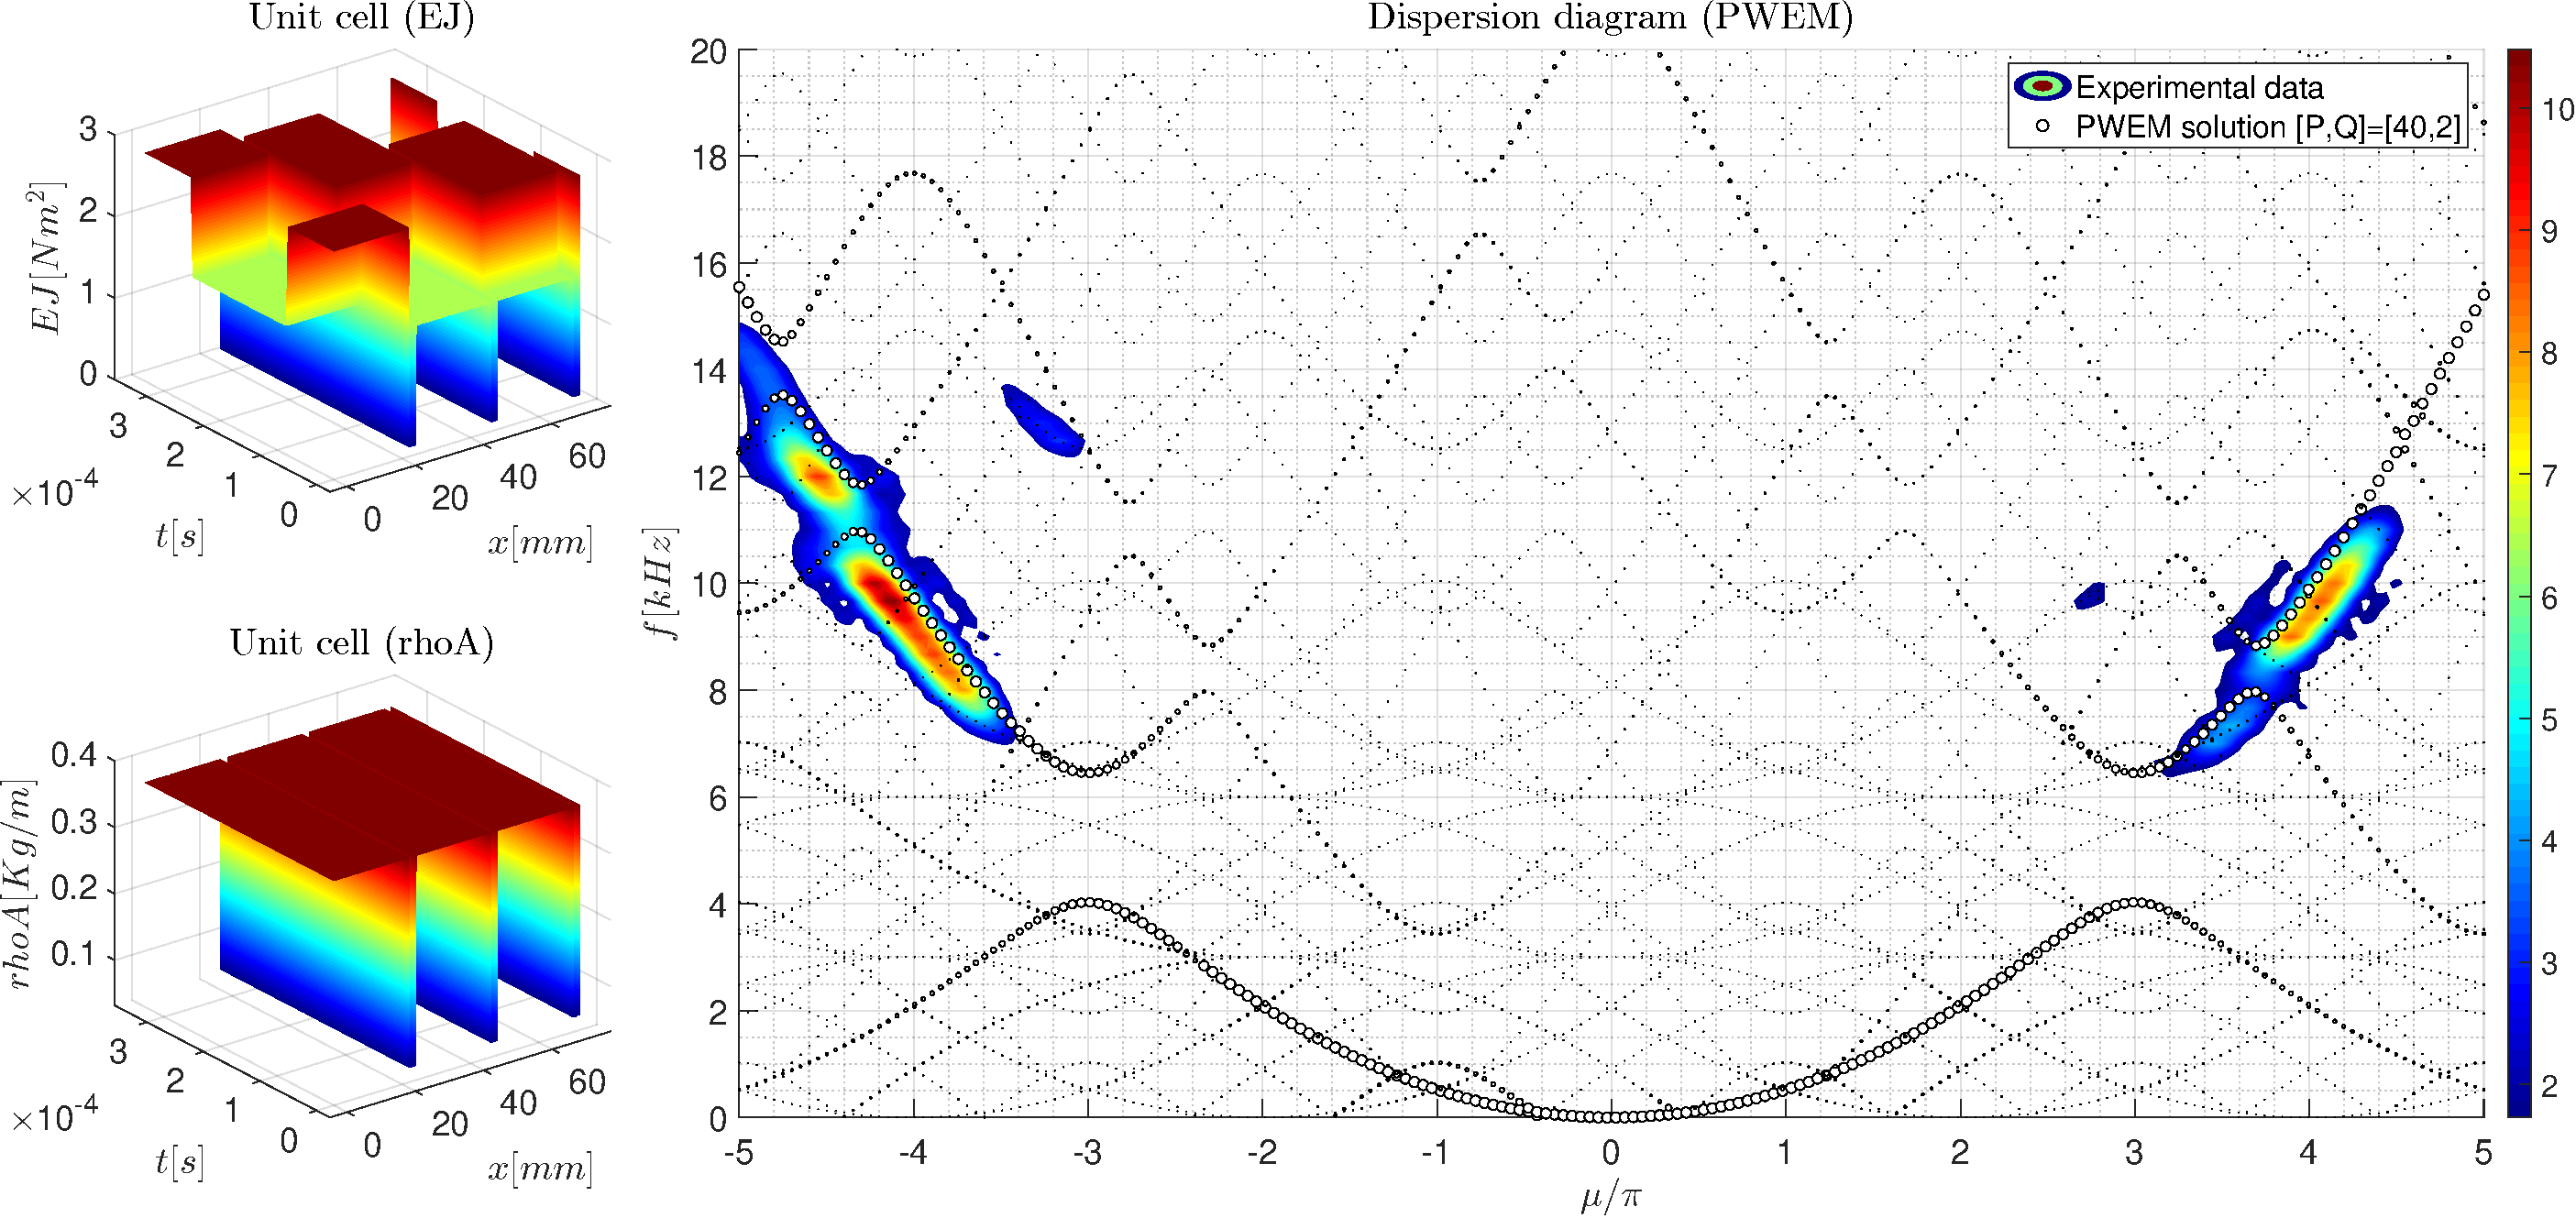
\includegraphics[width=\textwidth]{img/MATLAB/PWEM_EXP Sinusoidal (discrete) @3kHz.pdf}
        \caption{Dispersion diagram for the case of modulation frequency $f_m = \pm 3 kHz$.}
    \end{figure}

\end{frame}